\chapter{Low-side load control}\label{ch:loadcontrol}
%**********************************************
\section{Literature}\label{sec:loadcontrol_lit}
In this design notable factors that will affect the design will be outlined. The load that will be used is made up of 5 LEDs that will be designed in such a way so that together 100mA is drawn. The NMOS we are going to use is able to sink a maximum continuous drain current of 200mA \cite{NData}. A low side switch means that the "switching element" is place in between ground and the load.

\section{Design}\label{sec:loadcontrol_design}
Because 100mA is the maximum current a 2n7000 NMOS chip was deemed enough to be used as a switch for the load. To "turn on" the NMOS a 5V control signal will be used. To ensure that the gate of the NMOS can not float a pull down resistor will be used For a drain current of 100mA, according to the data sheet the $V_{DSon}$ voltage will be approximately 0.2V for a $V_{gs}$ of 5V \cite{NData}. The LED we are using has a typical forward bias voltage of 3.2V at 20mA \cite{LED}. To limit the current to 20mA ($7.2V-20mA*R_{shunt}=3.2V+0.2V$) a resistor of 190\textohm \ would be ideal ,but only 220\textohm's are available in the labs. The LEDs will be in series with the current limiting resistor. The LED-resistor units will then be placed in parallel to each other.
\section{Results}\label{sec:loadcontrol_results}
 \begin{figure}[!htb]
 \footnotesize
 \centering
    \begin{subfigure}[]{0.42\textwidth}
              \centering
  		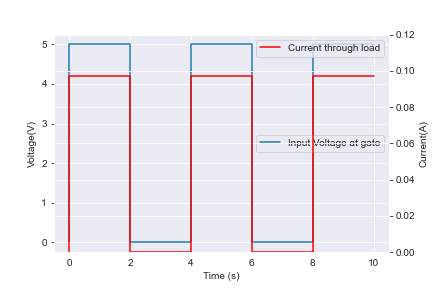
\includegraphics[width=1\linewidth]{./Figures/NMOS.png}
		    \caption{} \label{subfig:fig3}
     \end{subfigure}
     \begin{subfigure}[]{0.3\textwidth}
             \centering
  		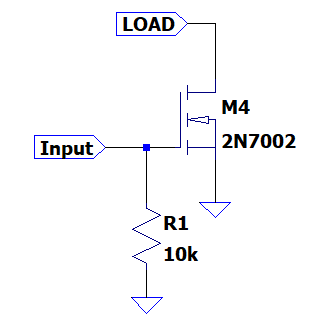
\includegraphics[width=1\linewidth]{./Figures/circNMOS.png}
		   \caption{ } \label{subfig:fig4}
     \end{subfigure}
   \caption[{Fuse Characteristics}]{NMOS final Results   (a)  LT Spice simulation (b) Basic Circuit }
    \label{fig:two}
 \end{figure}




\vfill

